\documentclass[11pt,a4paper,notitlepage,twocolumn]{article}

\usepackage[T1]{fontenc}
\usepackage[utf8]{inputenc}
\usepackage[english]{babel}
\usepackage{amsmath}
\usepackage{amsfonts}
\usepackage{amssymb}
\usepackage{verbatim}
\usepackage{listings}
\usepackage{color}
\usepackage{setspace}
\usepackage{epstopdf}
\usepackage{graphicx}
\usepackage{caption}
\usepackage{subcaption}
\usepackage{float}
\usepackage{epstopdf}
\usepackage{hyperref}
\usepackage{dsfont}
\usepackage{braket}
\pagenumbering{arabic}
\usepackage{titling}
\usepackage{fullpage}

\definecolor{codepurple}{rgb}{0.58,0,0.82}
\definecolor{backcolour}{rgb}{0.95,0.95,0.92}
\definecolor{dkgreen}{rgb}{0,0.6,0}
\definecolor{gray}{rgb}{0.5,0.5,0.5}
\definecolor{mauve}{rgb}{0.58,0,0.82}
%\setlength{\parindent}{0pt}

\lstdefinestyle{pystyle}{
  language=Python,
  aboveskip=3mm,
  belowskip=3mm,
  columns=flexible,
  basicstyle={\small\ttfamily},
  backgroundcolor=\color{backcolour},
  commentstyle=\color{dkgreen},
  keywordstyle=\color{magenta},
  numberstyle=\tiny\color{gray},
  stringstyle=\color{codepurple},
  basicstyle=\footnotesize,  
  breakatwhitespace=false
  breaklines=true,
  captionpos=b,
  keepspaces=true,
  numbers=left,
  numbersep=5pt,
  showspaces=false,
  showstringspaces=false,
  showtabs=false,
  tabsize=2
}
\lstdefinestyle{iStyle}{
  language=IDL,
  aboveskip=3mm,
  belowskip=3mm,
  columns=flexible,
  basicstyle={\small\ttfamily},
  backgroundcolor=\color{backcolour},
  commentstyle=\color{dkgreen},
  keywordstyle=\color{magenta},
  numberstyle=\tiny\color{gray},
  stringstyle=\color{codepurple},
  basicstyle=\footnotesize,  
  breakatwhitespace=false
  breaklines=true,
  captionpos=b,
  keepspaces=true,
  numbers=left,
  numbersep=5pt,
  showspaces=false,
  showstringspaces=false,
  showtabs=false,
  tabsize=2
}
\lstdefinestyle{c++style}{
  language=C++,
  keywordstyle=\color{blue}\ttfamily,
  stringstyle=\color{red}\ttfamily,
  commentstyle=\color{green}\ttfamily,
  morecomment=[l][\color{magenta}]{\#}
  aboveskip=3mm,
  belowskip=3mm,
  columns=flexible,
  basicstyle={\small\ttfamily},
  backgroundcolor=\color{backcolour},
  numberstyle=\tiny\color{gray},
  basicstyle=\footnotesize,  
  breakatwhitespace=false
  breaklines=true,
  captionpos=b,
  keepspaces=true,
  numbers=left,
  numbersep=5pt,
  showspaces=false,
  showstringspaces=false,
  showtabs=false,
  tabsize=2
}

\title{\normalsize Fys3150/4150 - Computational Physics\\
\vspace{10mm}
\huge 4. Ising model - Monte Carlo and Metropolis algorithms\\
\vspace{10mm}
\normalsize Due date {\bf Nov $overdue$, 2016}}

% Skriv namnet ditt her og fjern kommenteringa
\author{Magnus Christopher Bareid \\ un: magnucb }

\newcommand{\SE}{Schr\"odinger equation}
\newcommand{\laplacian}{\vec{\nabla}^2}
\newcommand{\eye}{\mathds{I}}
\newcommand\pd[2]{\frac{\partial #1}{\partial #2}}
\def\doubleunderline#1{\underline{\underline{#1}}}

\begin{document}
\noindent
\maketitle
\vspace{5mm}



%\begin{figure}[H]
%	\centering	
%	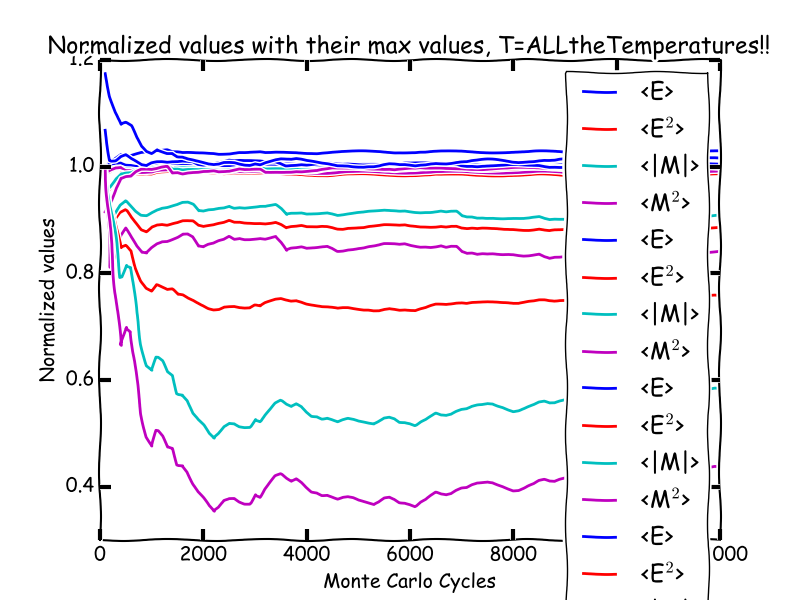
\includegraphics[scale=0.45]{frontpage.png}
%\end{figure}

\begin{abstract}
Empty void %TODO
\end{abstract}



%\begin{center}
%\line(1,0){450}
%\end{center}

\newpage
\tableofcontents

\newpage

\section{Studies of phase transitions in magnetic systems}
\subsection{Introduction}
The aim of this project is to study a widely popular model to simulate phase transitions, the so-called Ising model in two dimensions. At a given critical temperature, this model exhbits a phase transition from a magnetic phase (a system with a finite magnetic moment) to a phase with zero magnetization.

As with all other projects in this course, the important thing is to make the algorithm work. The basic energy calculation of any two-dimensional lattice boils down to this form:
\begin{align}\label{eq:energysummation}
E = -J \sum^N_{<kl>} s_ks_l
\end{align}
where $s_k$ and $s_l$ are $\pm 1$ (up or down spin), $N$ is the total spins in the lattice, $J$ expresses the strength of interaction between neighbouring spins, which are referred to in the summation by $<kl>$ as it sums up interaction only between lattice-neighbours near index $k$ and $l$.

Through the course of this report, we shall investigate different variations on differently-sized lattices and their modelled physical properties.

\subsection{Analytical model of $2\times2$ lattice}
For our first trick, we shall simply investigate a $2\times2$ lattice of spins and its properties: its expectation value for energy and for absolute magnetic moment (mean magnetization), its  specific heat and magnetic susceptibility.

\subsubsection{The underlying math}
Firsly, we'll bee needing the partition function
\begin{align}\label{eq:partitionfunc}
Z = \sum_i e^{-\beta E_i}
\end{align}
where $E_i$ is a spin configuration's energy level, which $i$ counts over, and $\beta = 1/(k_B T)$ as a physical variable depending on temperature - a parameter which will become important in later sections.

The lattice's energy is given from the same form as equation (\ref{eq:energysummation}). The magnetic moment of such a lattice's spin combination is also important, and will yield values in a similar, but different pattern to the energy variations. For this we use:
\begin{align}\label{eq:magnetsummation}
M = \sum_{i=1}^N s_i
\end{align}
where $M_i$ signifies a lattice location's spin orientation. This reveals to us a set of energies and magnetizations that the $2\times2$ lattice and its possible spin configurations may yield.
\begin{table}[H]
\center
\begin{tabular}{|c|c|r|r|} \hline

	\# $s_i=$ 1 & \# states & E & M  \\ \hline
	4 & 1 & -8J & 4   \\
	3 & 4 & 0   & 2   \\
	2 & 4 & 0   & 0   \\
	2 & 2 & 8J  & 0   \\
	1 & 4 & 0   & -2  \\
	0 & 1 & -8J & -4  \\ \hline
\end{tabular}
\caption{Overview over how number of spins in a direction determines energy and magnetization of a lattice, and its multiplicity.}\label{table:spincombinations}
\end{table}

For the related expectation values, these are formed by multiplying by the probability of each state, which is determined with a natural exponent and the partition function that we elaborated earlier:
\begin{align}\label{eq:exvals}
<E^n> &= \frac{1}{Z}\sum_i E_i^n e^{-\beta E_i}  \\
<|M|^n> &= \frac{1}{Z}\sum_i M_i^n e^{-\beta E_i} \nonumber
\end{align}
where $i$ iterates over all possible combinations - not over all locations in a lattice.

Furthermore, the formulation for specific heat and magnetic susceptibility reads thus:
\begin{align}\label{eq:specheat_magsus}
C_V &= \frac{<E^2> - <E>^2}{k_B T^2} \\
\chi &= \frac{<M^2> - <M>^2}{k_B T} \nonumber
\end{align}

\subsubsection{Results}
When all of these energy and magnetic combinations are input to a simple python script, the analytical values which we were supposed to investigate, as mentioned in the beginning of the section, may be evaluated:

\begin{table}[H]
\center
\begin{tabular}{|c|r r|}\hline
	$<E>$ &-7.98392834375   $\approx$ & -7.9839\\ \hline
	$<M>$ & 3.99464293099   $\approx$ & 3.9946\\ \hline
	$C_V$ & 0.128329327457  $\approx$ & 0.12833\\ \hline
	$\chi$& 0.0160429580649 $\approx$ & 0.016043\\ \hline
\end{tabular}
\caption{Analytical values as determined by a python script.}\label{table:analyticalresults}
\end{table}

\subsection{Making a working numerical model}
Now comes the fun part% DIE DIE DIE!!!!!!!!
, modelling the previous system numerically, using Monte Carlo style in C++.

\subsubsection{How the script works}
The script begins by taking in several values of the lattice system, such as lattice length, how many Monte Carlo cycles which we will cycle the system over, temperature for the lattice to hold. The temperature in this case is set to 1 for simplicity's sake. Physical units and confusions apply.

Then the inital lattice matrix is set up with corresponding energy and magnetization quantities; for this problem's purposes we simply start with all spins up.

At every iteration of the Monte Carlo cycle, the lattice is adjusted according to principles of physics: A random spin is chosen to turn its value. If the new energy state has less energy than the previous one, the new energy state is then accepted its new properties for energy and magnetization are applied to the system.

Expectation values are yielded from dividing by number of Monte Carlo cycles which the system has had to go through in order to achieve its current properties. The iterated values are stored to data files for later use, expectation values are printed to screen along with specific heat and magnetic susceptibility.

\subsubsection{Results and discussion}
A run for several Monte Carlo simulation lengths yielded these values, which are compared with analytical results as shown in table \ref{table:analyticalresults}.
\begin{table}[H]\center
\begin{tabular}{|c|r|r|}\hline
	Quant.& Result & $\approx\Delta$ Ana.\\ \hline
	$<E>$ &-7.2    & 0.7839 \\ \hline
	$<M>$ & 3.63   & 0.3646 \\ \hline
	$C_V$ & 5.76   & 5.632 \\ \hline
	$\chi$& 1.44   & 1.424 \\ \hline
\end{tabular}
\caption{Results after $10^1$ Monte Carlo cycles.}\label{table:4bresults10}
\begin{tabular}{|c|r|r|}\hline
	Quant.& Result & $\approx\Delta$ Ana.\\ \hline
	$<E>$ &-7.92   & 0.0639 \\ \hline
	$<M>$ & 3.96   & 0.0346 \\ \hline
	$C_V$ & 0.6336   & 0.5053 \\ \hline
	$\chi$& 0.1584   & 0.1423 \\ \hline
\end{tabular}
\caption{Results after $10^2$ Monte Carlo cycles.}\label{table:4bresults100}
\begin{tabular}{|c|r|r|}\hline
	Quant.& Result & $\approx\Delta$ Ana.\\ \hline
	$<E>$ &-7.984  & 0.0001 \\ \hline
	$<M>$ & 3.992  & 0.0026 \\ \hline
	$C_V$ & 0.127744 & 0.0006 \\ \hline
	$\chi$& 0.031936 & 0.0159 \\ \hline
\end{tabular}
\caption{Results after $10^3$ Monte Carlo cycles.}\label{table:4bresults1000}
\begin{tabular}{|c|r|r|}\hline
	Quant.& Result & $\approx\Delta$ Ana.\\ \hline
	$<E>$ &-7.9856    & 0.0017 \\ \hline
	$<M>$ & 3.995    & 0.0004 \\ \hline
	$C_V$ & 0.114993   & 0.0133 \\ \hline
	$\chi$& 0.015575   & 0.0005 \\ \hline
\end{tabular}
\caption{Results after $10^4$ Monte Carlo cycles.}\label{table:4bresults10000}
\begin{tabular}{|c|r|r|}\hline
	Quant.& Result & $\approx\Delta$ Ana\\ \hline
	$<E>$ &-7.982  & 0.0019 \\ \hline
	$<M>$ & 3.99396    & 0.0007 \\ \hline
	$C_V$ & 0.143676   & 0.0153 \\ \hline
	$\chi$& 0.0182035   & 0.0022 \\ \hline
\end{tabular}
\caption{Results after $10^5$ Monte Carlo cycles.}\label{table:4bresults100000}
\begin{tabular}{|c|r|r|}\hline
	Quant.& Result & $\approx\Delta$ Ana.\\ \hline
	$<E>$ &-7.98436 & 0.0004 \\ \hline
	$<M>$ & 3.99479 & 0.0001 \\ \hline
	$C_V$ & 0.124875 & 0.0035 \\ \hline
	$\chi$& 0.0156048 & 0.0004 \\ \hline
\end{tabular}
\caption{Results after $10^6$ Monte Carlo cycles.}\label{table:4bresults1000000}
\end{table}

It would seem that already after having passed 10$^3$ Monte Carlo cycles, the accuracy starts to become surprisingly impressive, and varies less. However, the clear trend is of course that the more one increases the number of cycles for the program to run through, the more accurate results. My own verdict would claim that any run of the script with more than 10$^6$ Monte Carlo cycles would be accurate enough for most purposes.

\section{Appendix}
\subsection{Code and GitHub}
All my code is located at this address:

\url{https://github.com/magnucb/p4}

\begin{thebibliography}{9}
\bibitem{example_code}
  Jensen, M 2016,
  \verb|ParaIsingModel.cpp|,
  
  viewed $22^{th}$ of November 2016,
  \url{https://github.com/CompPhysics/ComputationalPhysics/blob/master/doc/Programs/ParallelizationMPI/ParaIsingModel.cpp}.
  
\bibitem{analytical_methods}
	Jensen, M 2016, 
	Computational Physics Lecture Notes Fall 2015:
	
	13.2.2: Canonical Ensemble \& 
	
	13.3.1: Ising Model and Phase Transitions in Magnetic Systems,
	
	viewed $22^{th}$ of November 2016, 
	\url{http://compphysics.github.io/ComputationalPhysics/doc/Lectures/lectures2015.pdf}

\end{thebibliography}

\end{document}